\chapter{First readings on the new atlas}\label{ch:firstreadings}

\begin{keybox}[title=Status of everything in this chapter]
\preview. These readings come from the v2 reader before its acceptance tests have passed and before the switch-over. They show what the
instrument does on real arrays. They are not evidence about any person, cell type or condition, and no conclusion in this book rests on them.
\end{keybox}

\section{What was read}

Two sets of arrays, each through the chain's own Stage~1 from the raw IDATs, composition by the v2 solver, each present cell read on its v2
identity loci:
\begin{itemize}
\item 24 healthy whole-blood arrays from the Uppsala laboratory (GSE87571), ages 14 to 94;
\item 44 sorted fractions from bone-marrow aspirates of people with acute myeloid leukaemia (GSE63409~\cite{Jung2015}): 15 CD34$^-$, 15 CD34$^+$CD38$^+$
      and 14 CD34$^+$CD38$^-$.
\end{itemize}

\section{A first run that went wrong, and why}

The first run gave healthy blood a composition no haematologist would accept: the six bone-marrow progenitor populations took a large share of the mass,
and monocytes and B cells were starved. Progenitor profiles are broad and intermediate, so a least-squares solver can use a little of each to absorb small
misfits everywhere. A per-specimen scale term did not remove the effect. Removing progenitors from the candidate cells for circulating blood did. That is
now a rule by specimen type (Chapter~\ref{ch:separation}).

\section{Healthy whole blood}

\begin{figure}[t]\centering
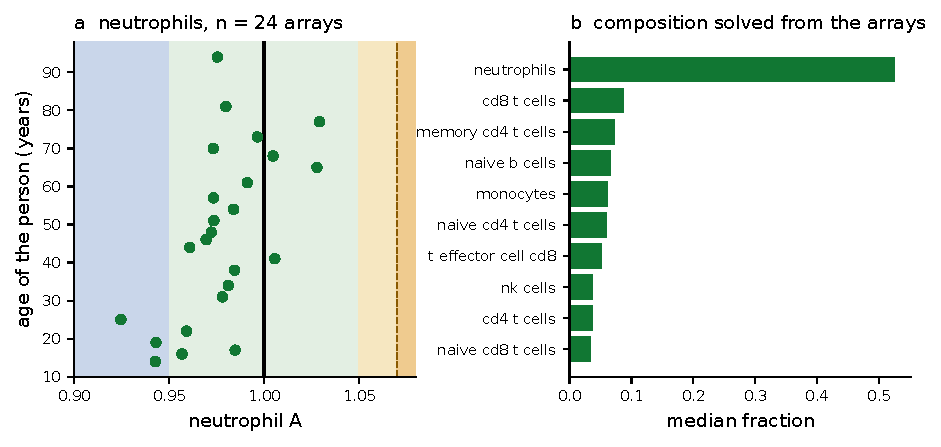
\includegraphics[width=\textwidth]{figures/part4/fig_run02.pdf}
\caption{Preview readings on 24 healthy whole-blood arrays (GSE87571) on atlas v2. (a) Neutrophil $A$ against the person's age, over the tier bands. (b) Median
fraction of the ten largest components. \preview}
\label{fig:run02}
\end{figure}

\paragraph{Composition.} Median neutrophils 53~\%, CD8 T cells 9~\% (and more in CD8 subsets), memory CD4 T cells 7~\%, naive B cells 7~\%, monocytes 6~\%,
naive CD4 T cells 6~\%, NK cells 4~\% (Figure~\ref{fig:run02}b). The progenitor sink is gone.

\paragraph{Neutrophils.} Median $A=0.977$; 21 of 24 in Normal; range 0.925--1.029. The three below Normal are from people aged 14, 19 and 25, and $A$ rises
with age across the 24 (correlation 0.58; Figure~\ref{fig:run02}a). \observed{} It agrees in direction with the author's statement that ageing raises $A$. It is
24 arrays from one laboratory on an uncommissioned reader, and it is an observation about where people of different ages sit on the gauge, which by the rule
of the front matter is never a correction to any cell.

\paragraph{Minor cells.} Monocytes read Normal on 22 of 24 arrays, NK cells on 18 of 19 where present, basophils on 21 of 22, eosinophils on 7 of 7. The T-cell
and B-cell subsets do not: naive CD4 T cells 3 of 16 in Normal (median 1.062), naive B cells 9 of 24 (1.055), memory CD4 T cells 2 of 19 (0.923). These are cells
at a few per cent that share much of their methylation with their neighbours, and Figure~\ref{fig:fracprec} predicts exactly this: at that fraction the error in
the other cells' fractions dominates the reading. \measured{} (for the counts; the explanation is \conjecture{} until tested by the pre-registered minor-cell
procedure).

\paragraph{A leak.} The embryonic stem cell profile took 1--2~\% of the mass in 15 of 24 healthy arrays. A pluripotent cell cannot be in adult blood. It is the same
kind of failure as the progenitor sink, and the fix is the same: the candidate set for circulating blood. \measured

\section{Sorted AML fractions}

In each sorted fraction the largest component was read as a GMP-like progenitor on 30 of 44 arrays, monocyte-like on 10, and L-MPP-like on 2. The largest
component's median $A$ was 1.035 (CD34$^+$CD38$^-$), 1.064 (CD34$^-$) and 1.065 (CD34$^+$CD38$^+$), with the highest reading 1.139. The residual after composition
was more than twice that of healthy blood (median absolute residual 0.077 against 0.032): these specimens are not well described by any mixture of healthy atlas cells.
\preview

That is the direction the framework predicts for a transformed cell population: toward $\beta=\tfrac12$ on the cell's identity loci. It is not yet a comparison anyone
should rely on. The healthy progenitors the AML cells are read against were in the atlas fit, and a fair reading needs healthy bone-marrow progenitors held out of the
atlas, read the same way, landing at 1.00. That is the first blood-cancer procedure in the plan.

\section{What these readings are for}

They show three things about the instrument, and nothing yet about people. The v2 reader runs end to end on raw arrays with no population-derived number. The
composition problems that remain are specific and nameable (candidate sets, subset collinearity, one leaking profile). And the readings on the major cells of healthy
blood land near the fixed point on a reference built from purified cells, with no whole-blood specimen and no population of readings used to set any number.
